% Use only LaTeX2e, calling the article.cls class and 12-point type.

\documentclass[12pt]{article}

% Users of the {thebibliography} environment or BibTeX should use the
% scicite.sty package, downloadable from *Science* at
% www.sciencemag.org/about/authors/prep/TeX_help/ .
% This package should properly format in-text
% reference calls and reference-list numbers.

\usepackage{booktabs}
\usepackage{graphicx}



% Use times if you have the font installed; otherwise, comment out the
% following line.

\usepackage{times}
\usepackage{float}

% The preamble here sets up a lot of new/revised commands and
% environments.  It's annoying, but please do *not* try to strip these
% out into a separate .sty file (which could lead to the loss of some
% information when we convert the file to other formats).  Instead, keep
% them in the preamble of your main LaTeX source file.


% The following parameters seem to provide a reasonable page setup.

\topmargin 0.0cm
\oddsidemargin 0.2cm
\textwidth 16cm 
\textheight 21cm
\footskip 1.0cm


%The next command sets up an environment for the abstract to your paper.

\newenvironment{sciabstract}{%
\begin{quote} \bf}
{\end{quote}}


% If your reference list includes text notes as well as references,
% include the following line; otherwise, comment it out.

\renewcommand\refname{References and Notes}

% The following lines set up an environment for the last note in the
% reference list, which commonly includes acknowledgments of funding,
% help, etc.  It's intended for users of BibTeX or the {thebibliography}
% environment.  Users who are hand-coding their references at the end
% using a list environment such as {enumerate} can simply add another
% item at the end, and it will be numbered automatically.

\newcounter{lastnote}
\newenvironment{scilastnote}{%
\setcounter{lastnote}{\value{enumiv}}%
\addtocounter{lastnote}{+1}%
\begin{list}%
{\arabic{lastnote}.}
{\setlength{\leftmargin}{.22in}}
{\setlength{\labelsep}{.5em}}}
{\end{list}}


% Include your paper's title here

\title{Machine Learning for Human Activity Recognition} 


% Place the author information here.  Please hand-code the contact
% information and notecalls; do *not* use \footnote commands.  Let the
% author contact information appear immediately below the author names
% as shown.  We would also prefer that you don't change the type-size
% settings shown here.

\author
{Thomas~Wolfe, Aditya~Subramanian, Shairoz~Sohail\\
\\
\normalsize{Department of Statistics, University of Illinois Urbana-Champaign}\\
\
}

% Include the date command, but leave its argument blank.

\date{}



%%%%%%%%%%%%%%%%% END OF PREAMBLE %%%%%%%%%%%%%%%%



\begin{document} 

% Double-space the manuscript.

\baselineskip24pt

% Make the title.

\maketitle 



% Place your abstract within the special {sciabstract} environment.

\begin{sciabstract}
  Being able to provide users with an accurate representation of their actions at any given point of time, based off of sensor data modeled through a mobile device is required to personalize user actions per individual. Based on gyroscope and accelerometer data collected, as well as other heuristics which are described in latter parts of the paper. We integrate supervised machine learning algorithms, including clustering, regression, and classification algorithms.
Our end goal, of observing the differences between users for different activities based on the mode,l was applied to walking, sitting, and standing, lying down, and different variations of the aforementioned activities. 
\end{sciabstract}



% In setting up this template for *Science* papers, we've used both
% the \section* command and the \paragraph* command for topical
% divisions.  Which you use will of course depend on the type of paper
% you're writing.  Review Articles tend to have displayed headings, for
% which \section* is more appropriate; Research Articles, when they have
% formal topical divisions at all, tend to signal them with bold text
% that runs into the paragraph, for which \paragraph* is the right
% choice.  Either way, use the asterisk (*) modifier, as shown, to
% suppress numbering.

\section*{Introduction}

The analysis of human movement data is becoming an increasingly important application in modern technologies. From video game peripherals that let you interact with game elements, to smartwatches and activity trackers that can help you manage your health; accuracy in movement detection is paramount. For this paper we look at the Human Activity Recognition (HAR) using smartphones dataset, hosted at the University of California, Irving website. There are a few analysis already performed on this dataset \cite{anguita2012human}, with a maximum activity classification accuracy of 96\%. We aim to reach or surpass this accuracy while keeping in mind computational cost, as most applications of activity recognition depend on quick and dynamic output. We also explore a large variety of different models and software packages during the process to attempt to uncover new insights into performance between models/packages.

\subsection{Data Collection}
The data used in this analysis came from a group of 30 volunteers aged 19-48 years old. Each volunteer wore a Galaxy S2 smartphone attached to their waists and performed the six different activities (Walking, Walking Upstairs, Walking Downstairs, Sitting, Standing, and Laying) \cite{anguita2012human}. The Galaxy S2 was used for this experiment because it contained an accelerometer and a gyroscope for measuring 3-axial linear acceleration and angular velocity respectively at a constant rate of 50Hz, which is adequate for capturing human body motion \cite{anguita2012human}. 
    
A smartphone application was used to acquire the sensor signal and these signals were pre-processed by applying noise filters and then were sampled in fixed-width sliding windows of 2.56 sec and 50\% overlap \cite{anguita2012human}. For each 2.56 sec window, a vector of 17 features was obtained by calculating variables from the accelerometer signals in the time and frequency domain \cite{anguita2012human}. Then, Fast Fourier Transform was used to find the signal frequency components \cite{anguita2012human}. Lastly, the patterns found were then used to train the following models.

\subsection{Data Structure}
The data is randomly split into two data sets, one set has 70\% of the patterns and is used for training the models. The other 30\% of the patterns is used to determine how accurate the model is. There are 561 features and each row of data has the following included:

-Triaxial acceleration from the Galaxy S2’s accelerometer (total acceleration) and the estimated body acceleration

- Triaxial Angular velocity from the Galaxy S2’s gyroscope

- A 561-feature vector with time and frequency domain variables. 

- The activity label (Walking, Walking Upstairs, Walking Downstairs, Sitting, Standing, or Lying)

- A subject identifier

\subsection{Pre-Processing}
The data was already scaled to [0,1] and strong outliers removed. We performed an additional Z-Scaling (removing mean and dividing by the standard deviation) as well as a removal of correlated predictors.

An important aspect of our data to note is that being gyroscopic data, many of our measurements were repetitive or highly correlated. With the number of sensors and small amount of movements represented (six) we found a large number of correlated predictors (288) and removed them. This accounts for a removal of over 50\% of our predictors, a number that seems high but is justified via the means of data collection and strict correlation cutoff (0.95). 

The remaining predictors all have non-zero variance and are thus useful for modeling. We provide a visual of the categories in our remaining dataset below.
\begin{figure}[h]
\caption{Activity Counts}
\centering
{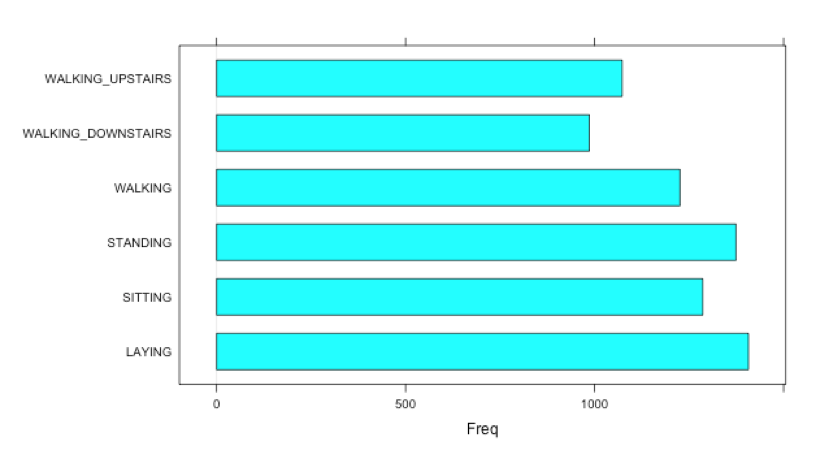
\includegraphics[width=4in,height=4in,keepaspectratio]{preproc}}
\end{figure}


\section{Materials \& Methods}
Initial portions of model fitting required experimentation with baseline models to ultimately determine the style of the data. 

Through experimentation and implementation, we decided on the below supervised machine learning algorithms to distinguish the various gestures from one another. 

\subsection{Discriminant Analysis}
We aim to classify our gyroscope measurements into an activity class. Discriminant Analysis is a procedure that aims to express the response category as a linear combination of the features. In this sense it is similar to Logistic Regression, but in Discriminant Analysis we take advantage of Bayes Theorem.

Let be the population distribution of the ith class. Then, for Linear Discriminant Analysis we model each  as multivariate normal with mean vector μi and variance-covariance matrix Σ (same for all populations). As a formula, this is:
$$f(\mathbf{x}|\pi_i) = \frac{1}{(2\pi)^{p/2}|\mathbf{\Sigma}|^{1/2}}\exp\left[-\frac{1}{2}\mathbf{(x-\mu_i)‘\Sigma^{-1}(x-\mu_i)}\right]$$
We classify to the population for which $f(\mathbf{x}|\pi_i)$ is largest using Bayes Theorem. Since the variance-covariance matrix $\Sigma$ will be independent of the population from which the data is obtained, we may take a log-transform (since it is monotonic and preserves maxima) and re-format the equation into one that depends only on the pooled variance-covariance matrix and each of the population means $\mu‘_i$, this is called the Linear Discriminant Function:
$$d^L_i(\mathbf{x}) = -\frac{1}{2}\mathbf{\mu‘_i\Sigma^{-1}\mu_i + \mu‘_i\Sigma^{-1}x} = d_{i0} + \sum_{j=1}^{p}d_{ij}x_j$$

This procedure will not work well if the population distributions for each class are not roughly Gaussian.\cite{IEEE} The importance of applying this procedure first is to gauge the nature of the relationship between the predictors and response. Comparing the performance of Linear Discriminant Analysis to more flexible methods like Random Forest will allow us to get a feeling of the relationship between the predictors (gyroscope measurements) and response (activity) and tell us whether to try the wide range of linear modeling techniques or explore the somewhat more complicated areas of modeling highly non-linear relationships.



\subsection{Multinomial Regression}
Due to the high performance of the previous Linear Discriminant Analysis, further linear models such as the Multinomial Regression were used. This method is a generalization of Logistic Regression to account for multiple output classes, and such is the case with our data. While the method itself is quite extensive, it serves as modeling the probability of an observation i being in class , given a vector of predictors X

$$ p(Y_{i} = k | X_i= (x_{1}, x_{2}, \ldots x_{n})) $$

\subsection{Random Forest}
Random Forest uses the concept of ensemble learning which leverages the power of several weak learners to make more accurate predictions. Random Forests implement the previous concept by building a set of decision trees. Each decision tree randomly selects from the features and the overall sample space. Then, the predictions from the trees are combined to make a final prediction. In order to prevent overfitting Random Forests use a bagging technique. A bagging technique ensures that when the algorithm builds new decision trees it will not look analyze previous trees.

A Random Forest model is implemented for this data set because it is capable of handling a large number of features and it makes no assumptions about the data. 


\subsection{Gaussian Naive Bayes}
The Naive Bayes algorithm is an implementation of Bayes theorem using a prior assumption that all incoming features are independent of one another. 

$$P(x_i | y) = 1\frac{1}{\sqrt{2\pi\sigma^{2}_y}}\exp(-\frac{(x_i - \mu_y)^2}{2\sigma^2_y})$$


Using maximum likelihood estimates to derive parameters σy and μy a maximum likelihood is iteratively taken, representative for individual, unique points.  The conditional probability measurement taken to derive final accuracy behind the classifier allows for the model to work comparatively quickly. However, this results in a mathematically unstable estimator, depending on the type of data which is inputted to the algorithm. 

\subsection{KNN (N = 10)}
We used an iterative k-Nearest Neighbors method, a clustering algorithm used to group data into centroids. The KNN algorithm, has a default centroid set to N = 5.  We used an iterative approach to decide which centroid count would be most optimal for the overall accuracy. Each iteration increased the count of the centroids from 5 to 10, and saw if there was overall trend in the accuracy. Observing a decrease in misclassification rates, the centroids were set to N = 10. 

This approach for identifying clusters was a brute force attack. However, the variability in the accuracy was less than 1\% overall between iterative clusters. Further, we ensured that a global maximum and global minimum of the accuracy was met before allowing the value to stay at N = 10. These methods allowed for us to confirm that the amount of neighbors was not as significant in the overall accuracy, as the change was around 1\%, given the difference in centroids. 

\subsection{Linear Support Vector Classification}
The linear support vector classifier is a support vector classifier with an underlying linear kernel. The linear method is helpful for deciding decision boundaries based off of minimizing the error residual between points. 

\subsection{Stochastic Gradient Descent}
Stochastic gradient descent is an algorithmic approach of minimizing the loss rate between any two data points. The algorithm iteratively steps through a myriad of points, and objectifies the data with the largest difference between two indices. Those points with large data gaps between themselves are marked as belonging towards different functions, and are not related on their own to one another. 

\section{Analysis}
Baseline models of Linear Discriminant Analysis, as well as multinomial regression and random forests allowed for us to gauge the veracity of the data set. In order to further extrapolate on the linear characteristics and trends extracted from the baseline results, a Linear Support Vector Classifier was one of the first methods used. This method ultimately boasted one of the highest accuracies, around 96\%. 
	Of the classifications in the Linear Support Vector Classifier (LSVC), a confusion matrix was used to understand where the loss of accuracy could be attributed towards. 
\begin{figure}[H]
\caption{LSVC Confusion Matrix}
\centering
{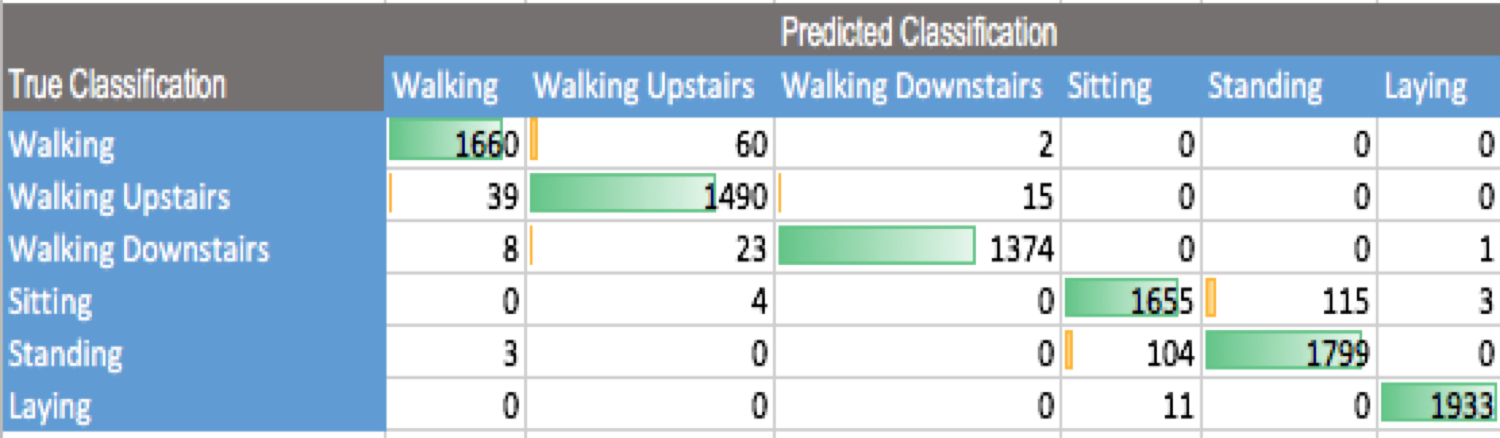
\includegraphics[width=4in,height=4in,keepaspectratio]{LSVCConf}}
\end{figure}
\noindent {\bf Fig. 2.} The green bars represent the proportion of proper estimation by the algorithms. On the contrary, the yellow bars represent the proportion of misclassified labels.
	
	
	
	The confusion matrix shows distinct areas where the yellow misclassification margins are relatively larger. The first of these two instances is around the walking portions. Differentiating the activity from walking, versus walking upstairs or walking downstairs became a technically complicated problem to solve. In particular, differentiating an individual from walking downstairs, walking upstairs, or walking on level ground requires information regarding the z-axis, and respective gyroscopic movements. Furthermore, the differentiation between the z-axis is only as relevant as the timestamp associated with each point. The time stamp would allow for the understanding of the data progression, and how the stages changed at any given point. Unfortunately, the data was not coupled with time progression as usable metric. Being able to understand said progression would be able to relieve the relatively few misclassified errors found here. 
	
	Furthermore, another instance of confusion could be found between standing or sitting. This confusion can be traced back to the data acquisition section of the methods. During this acquisition phase, individuals have a Samsung Galaxy S2 phone mounted on their waist. From standing or sitting down, there would only be a slight change in the position, as well as the z-axis. This comes to the same problem as with the walking upstairs or walking downstairs, where the lack of z-axis direction causes for a misguided approach to the problem. Being able to annotate, and appropriate for this misclassification would be found in the description of the data set, and pertaining documents. 
	
	It is important to note however, that unrelated activities are not misclassified as one another. In particular, activities like Laying and Walking are not misclassified, and the linear boundaries constructed by the Linear SVC are rigid enough to cover these boundaries. 
	
	Of the remaining models which were run, it was pertinent that models fitting a linear trend were better suited for the data set, where as other classification and regression methods performed with lower accuracies. In example, the naive bayes classifier, where each observation is observed as independent from the previous data point, performed with the lowest accuracy of around 73\%. This was to say that the information per data point did not fit into any specific trend, and was therefore discarded when analyzed algorithmically. 

\section{Conclusion/Discussion}
\subsection{Results}
Table 1 below depicts accuracy and algorithm information pertaining to the various classification techniques used for the problem. We can see that Linear SVC has the highest accuracy, followed closely by Multinomial Regression. The remaining classifiers, type of algorithm, adjusted parameters, iterations, and accuracy are all listed as well\cite{github}. 
\begin{table}[H]
\centering
\caption{Model Results}
\label{my-label}
\begin{tabular}{@{}lllll@{}}
\toprule
Model                            & Type                         & Parameters & Iterations &  Accuracy                                               \\ \midrule
LSVC  & Classification               & Default    & 10         & \begin{tabular}[c]{@{}l@{}}96.127 \\ $\pm$1.736E-2\end{tabular} \\
                                 &                              &            &            &                                                             \\
Multinomial Regression           & Regression                   & Default    & 10         & \begin{tabular}[c]{@{}l@{}}95.711\\$\pm$1.963E-2\end{tabular}  \\
                                 &                              &            &            &                                                             \\
K-Nearest Neighbors              & Clustering                   & K=10     & 10         & \begin{tabular}[c]{@{}l@{}}90.504\\ $\pm$1.240E-2\end{tabular}  \\
                                 &                              &            &            &                                                             \\
Random Forest                    & Clustering                   & Default    & 10         & \begin{tabular}[c]{@{}l@{}}91.311\\ $\pm$1.976E-2\end{tabular}  \\
                                 &                              &            &            &                                                             \\
Stochastic Gradient Des.      & Optimization                 & Default    & 10         & \begin{tabular}[c]{@{}l@{}}89.455\\ $\pm$6.934E-2\end{tabular}   \\
                                 &                              &            &            &                                                             \\
Gaussian Naive Bayes             & Probabilistic  & Default    & 10         & \begin{tabular}[c]{@{}l@{}}72.695 \\$\pm$2.923E-2\end{tabular} \\ \bottomrule
\end{tabular}
\end{table}


\subsection{Principal Component Analysis}
An important dimensionality-reduction method is called Principal Components Analysis. This method models the vector of predictors as a sequence of uncorrelated and orthogonal vectors known as “Principle Components”. The construction of these principal components is based on capturing the maximum amount of variance in our dataset. We illustrate the effectiveness of this on our dataset with a comparison of number of Principal Components vs Variance Explained below:
\begin{figure}[H]
\caption{PCA Analysis}
\centering
{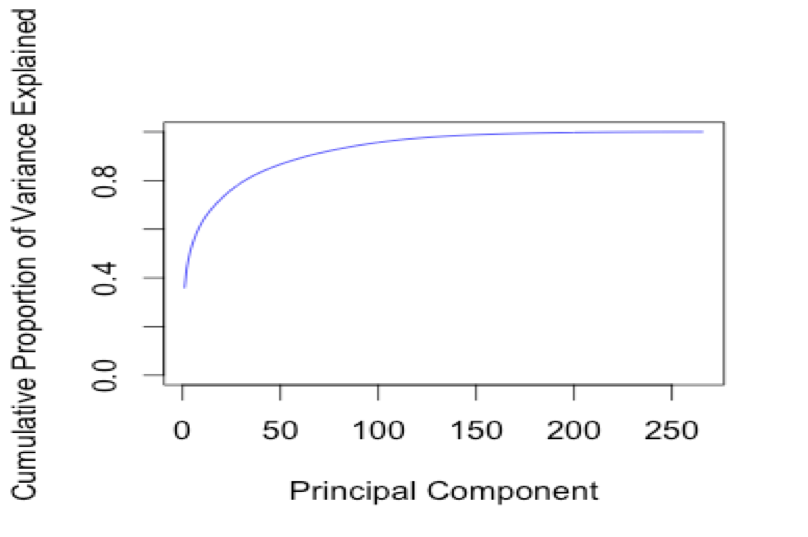
\includegraphics[width=4in,height=4in,keepaspectratio]{PCAS}}
\end{figure}
\noindent {\bf Fig. 3.} From this graph we can deduce that using $\sim$100 Principal Components will allow us to capture almost 95\% of the variance in our data. While we reduced the number of predictors significantly already (over 50\%), the use of Principal Components would allow us to reduce this number even further. Some of the challenges of using Principle Components come in the form of interpretability. \\
The Principle Components do not share the same scale or distribution as our original data, and thus using results for further modeling or pipelining into other applications (as is common with movement data) would be significantly hindered. 

\subsection{Cluster Analysis}
A huge problem in the field of human activity recognition is identifying new movements. Applications of HAR such as smart watches and fitness trackers rely on the device being able to discern a number of movements straight from production and not misclassifying new movements. The lack of user input in such applications provides us with an unsupervised learning framework. One of the most common methods in this area is clustering, separating data into clusters based on similar predictor values. Since we have labels for our data and it was collected in an experimental fashion, it is not really primed for unsupervised methods. However, we can apply a semi-unsupervised method known as K-Means Clustering by choosing K as the number of labels in our data set (six) and omitting the labels. Then we may check our clusters against the omitted labels to see how good our separation is.

\section*{Acknowledgments}
\noindent
Dr. Prashant Mehta $|$ Rithmio, Inc.\\
\noindent
Dr. Uma Ravat $|$ Department of Statistics $|$ University of Illinois at Urbana-Champaign \\
\noindent
University of California at Irvine $|$ Machine Learning Repository\\
\noindent
PIC Math is a program of the Mathematical Association of America (MAA) and the Society for Industrial and Applied Mathematics (SIAM).  
Support is provided by the National Science Foundation (NSF grant DMS-1345499)



\bibliographystyle{unsrt}
\bibliography{scibib}











\clearpage




\end{document}




















